\title{Solutions for Homework 6}
\author{Dr. Jordan Hanson - Whittier College Dept. of Physics and Astronomy}
\date{\today}
\documentclass[10pt]{article}
\usepackage[a4paper, total={18cm, 27cm}]{geometry}
\usepackage{graphicx}
\usepackage{amsmath}
\usepackage{tcolorbox}

\def\rcurs{{\mbox{$\resizebox{.16in}{.08in}{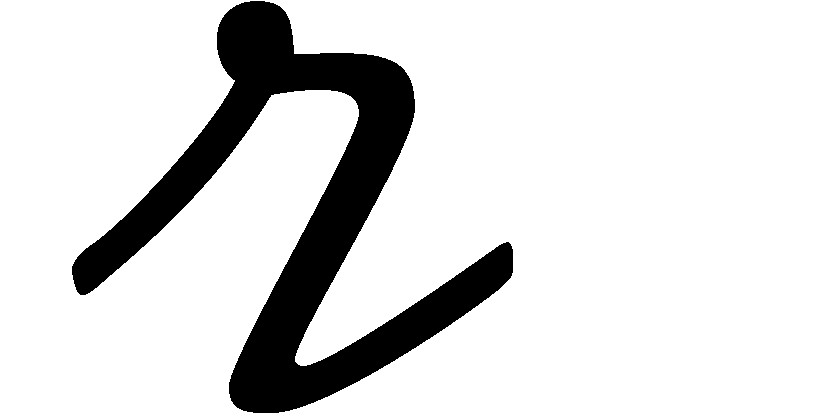
\includegraphics{ScriptR}}$}}}
\def\brcurs{{\mbox{$\resizebox{.16in}{.08in}{
\includegraphics{BoldR}}$}}}
\def\hrcurs{{\mbox{$\hat \rcurs$}}}

\begin{document}
\maketitle

\section{Problem 6.3}

\textit{Find the force of attraction between two magnetic dipoles, $\mathbf{m}_1$ and $\mathbf{m}_2$, oriented as shown in Fig. 6.7, a distance $r$ apart, (a) using Equation 6.2, and (b) using Equation 6.3.} \\ \\
The dipole moments are parallel to each other, and separated by a distance $r$.
\begin{itemize}
\item (a) Equation 6.2 says that $F = 2\pi I R B\cos\theta$.  Let $B\cos\theta = \mathbf{B} \cdot \hat{\mathbf{y}}$ (Fig. \ref{fig:1}), and The $\mathbf{B}$-field of $\mathbf{m}_1$ is 
\begin{equation}
\mathbf{B} = \frac{\mu_0}{4\pi}~\frac{3(\mathbf{m}_1 \cdot \hat{\mathbf{r}})\hat{\mathbf{r}} - \mathbf{m}_1}{r^3}
\end{equation}
So multiplying both sides by $\hat{\mathbf{y}}$ ($\mathbf{B} \cdot \hat{\mathbf{y}}$) gives
\begin{equation}
B\cos\theta = \frac{\mu_0}{4\pi}~\frac{3(\mathbf{m}_1 \cdot \hat{\mathbf{r}})\hat{\mathbf{r}} \cdot \hat{\mathbf{y}} - \mathbf{m}_1 \cdot \hat{\mathbf{y}}}{r^3} = \frac{\mu_0}{4\pi}~\frac{3m_1\cos\phi\sin\phi}{r^3}
\end{equation}
Using $m_2 = \pi I R^2$, and Fig. \ref{fig:1}, we can show that
\begin{equation}
F = \frac{3\mu_0}{2\pi}m_1 m_2 \frac{\sqrt{R^2 - r^2}}{r^5} \to \frac{3\mu_0}{2\pi}m_1 m_2 \frac{1}{r^4}
\end{equation}
In the last step, we have applied $R \ll r$ for microscopic dipoles.
\item (b) Using Equation 6.3:
\begin{equation}
\mathbf{F} = \nabla (\mathbf{m}_2 \cdot \mathbf{B}) = (\mathbf{m}_2 \cdot \nabla) \mathbf{B} =  m_2 \frac{d}{dz}\left( \frac{\mu_0}{4\pi}\frac{1}{z^3} (3(\mathbf{m}_1 \cdot \hat{\mathbf{z}})\hat{\mathbf{z}} - \mathbf{m_1}) \right)
\end{equation}
The dipole moments are constant vectors in the $z$-direction.  Taking the derivative with respect to $z$, we find
\begin{equation}
\mathbf{F} = -\frac{3\mu_0}{2\pi}\frac{m_1 m_2}{r^4}\hat{\mathbf{z}}
\end{equation}
\begin{figure}[ht]
\centering
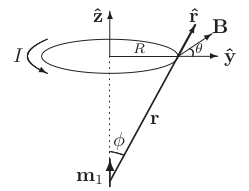
\includegraphics[width=0.25\textwidth]{dipole.png}
\caption{\label{fig:1} Diagram for Problem 6.3 (a).}
\end{figure}
\end{itemize}

\section{Problem 6.7}

\textit{An infinitely long circular cylinder carries a uniform magnetization $\mathbf{M}$ parallel to its axis.  Find the magnetic field (due to $\mathbf{M}$) inside and outside the cylinder.} \\ \\
The curl of a constant magnetization vector is zero, but there is a bound surface current:
\begin{equation}
\mathbf{K}_b = \nabla \times \hat{\mathbf{n}} = M\hat{\phi}
\end{equation}
But if this surface current is strictly circumferential, then that's a solenoid.  The field outside the solenoid is zero, and the field inside should be proportional to $M$.  Using the standard solenoid formula:
\begin{equation}
\mathbf{B} = \mu_0 K_b \hat{\mathbf{z}} = \mu_0 \mathbf{M}
\end{equation}

\section{Problem 6.16}

\textit{A coaxial cable consists of two very long cylindrical tubes, separated by linear insulating material of magnetic susceptibility, $\chi_m$.  A current $I$ flows down the inner conductor and returns along the outer one; in each case, the current distributes itself uniformly over the surface.  Find the magnetic field in the region between the tubes.}

\begin{align}
\oint \mathbf{H} \cdot d\mathbf{l} &= I_{\rm f,enc} \\
\mathbf{H} &= \frac{I}{2\pi s}\hat{\mathbf{\phi}}  \\
\mathbf{B} &= \mu_0(1+\chi_m) \mathbf{H} \\
\mathbf{B} &= \frac{\mu_0(1+\chi_m) I}{2\pi s}\hat{\mathbf{\phi}}
\end{align}

Using the standard formulas for bound current density and surface currents, we find that there is no bound $\mathbf{J}$, but there are bound surface currents.  Using Amp\`{e}re's Law with these currents gives the same field.

\end{document}

